%!TEX root = mb.tex



\section{Cryptographic Building Blocks}
\label{sec:buildingblocks}

In this section we present the building blocks \sys relies on.
Symmetric-key encryption (based on AES) is well known, and we do not discuss it here. Instead, we briefly discuss KeywordMatch (introduced by~\cite{blindbox}, to which we refer the reader for details) and more extensively discuss PrefixMatch, a new cryptographic scheme we designed for this setting.
When describing these schemes we refer to the encryptor as the gateway whose secret key is $k$ and to the entity computing on the encrypted data as the service provider (SP).


\subsection{KeywordMatch}\label{s:kwmatch}


KeywordMatch allows detecting if an encrypted keyword matches an encrypted data item by equality.
For example, given an encryption of the keyword ``malicious'', and a list of encrypted strings  [$\Enc$(``alice''), $\Enc$(``malicious''), $\Enc$(``alice'')], SP can  detect that the keyword matches the second string. 
For  this, we use a searchable encryption scheme~\cite{song:search, blindbox}.
Using this scheme, the gateway can encrypt a value $v$ into $\enc(v)$ and a rule $r$ into $\encr$ and SP can detect if there is a match between $v$ and $r$. 
 The security of searchable encryption is well studied~\cite{song:search, blindbox}: at a high level,  given a list of encrypted strings, and an encrypted keyword, SP does not learn anything about the encrypted strings, other than which strings match the keyword. 
 The encryption of the strings is {\em randomized}, so it does not leak whether two encrypted strings are equal to each other, unless, of course, they both match the encrypted keyword. 
  We use the technique from~\cite{blindbox}.

%!TEX root = mb.tex

%\section{Building block: Range match}
%An important operation over an encrypted packet is to determine if an encrypted field in the packet falls in an encrypted range.
%We will use the firewall as an example. 
%Consider the following firewall rule:
%
%Constructing an encryption scheme that allows checking if an encrypted value is in an encrypted range, has been a challenge in the applied cryptography community. The reason is that ..
%
%\begin{itemize}
%\item preserve the order between Encryptd values
%\item candidate: OPE
%\item candidate: mOPE
%\item So none of the existing schemes are satisfactory. A new scheme \RM.
%\end{itemize}
%
%\RM applies to cases when we know an upper bound on the values encrypted with OPE and this is a small number of values (say, less than 10,000).
%
%The small number of values permits us to improve in two ways over mOPE [1]
%No more interaction. We store the tree in mOPE on the gateway (client) side, which means that the gateway can compute a new encryption by itself without help from service provider. The storage at the gateway will remain small.
%Rare updates to ciphertexts. We can space out the ciphertexts of the values encrypted sufficiently. 
%
%This also enjoys a stronger security than OPE! It leaks less than order.
%The reason is that, the server does not learn the order between the values in packets, and only whether they map between two values in the rules. 
%
%this one is new
%
%discuss 
%
%would be good to explain the challenge from the 
%
%\todo{a more interesting name to the scheme}
%
%prefix gets mapped into interval, at most a certain number
%
%talk about building certain data structures that all works the same
%
%firewall need not change 

\subsection{PrefixMatch} \label{sec:range}

Many middleboxes perform detection over a {\it range} of port numbers or IP addresses. For example, a network administrator might wish to block access to all servers hosted by MIT, in which case the administrator would block access to the prefix 18.0.0.0/8, \ie{}, 18.0.0.0-18.255.255.255. PrefixMatch enables a middlebox to tell whether an IP address $v$ lies in between a range $[s_1, e_1)$, where $s_1$ = 18.0.0.0 and $e_1$ = 19.0.0.0; however, the middlebox does not learn the values of $v$, $s_1$, or $e_1$.
Unlike KeywordMatch, PrefixMatch is a new scheme we designed specifically for our setting.

One might ask whether PrefixMatch is necessary, or one can instead employ KeywordMatch using the same expansion technique we used for some (but not all) regexps in \S\ref{sec:bbarch}. 
To detect whether an IP address is in a range, one could enumerate all IP addresses in that range and perform an equality check. However, the overhead of using this technique for common network ranges such as firewall rules is prohibitive.
For our own department network, doing so would convert our IPv6 and IPv4 firewall rule set of only 97 range-based rules to $2^{238}$ exact-match only rules; looking only at IPv4 rules would still lead to 38M exact-match rules.
Hence, to perform typical middlebox behaviors {\it in practice}, we require a PrefixMatch scheme which is more efficient.

\subsubsection{Requirements}
The functionality of our PrefixMatch scheme is to encrypt a set of ranges $[s_1, e_1)$, $\dots$, $[s_n, e_n)$ into a set of prefixes $\Enc(s_1, e_1)$, $\dots$, $\Enc(s_m, e_m)$ ($m \geq n$), and a value $v$ into $\Enc(v)$, such that anyone with access to these encryptions can determine in which range $v$ lies, while not learning the values of $s_1$, $e_1$, $\dots$, $s_n$, $e_n$, and $v$. 
For concreteness, we explain our scheme by considering $v$, $e_i$ and $s_i$ as IP addresses, although the scheme supports ports as well.

\raluca{what happens to the security of ports, do we still need IPv6?}

Our goal in designing PrefixMatch was for it to be both efficient/fast {\em and} to provide strong security.

In terms of performance, both encryption (performed at the gateway) and detection (performed at the middlebox) should be practical for typical middlebox line rates.
Our PrefixMatch encrypts in $< 0.5\mu$s per value (we evaluate in \S\ref{sec:eval}).
Our design performs comparison between encrypted values and an encrypted rule (performed at the middlebox) using only on normal $\leq$/$\geq$ operators; hence it is compatible with existing classification algorithms such as tries, area-based quadtrees, FIS-trees, or hardware-based algorithms~\cite{packet_classif}.

For security, we require that the encryption scheme  not leak $v$ to SP.
SP must not learn anything about $v$ other than what interval it matches to. 
In  particular, even if $v_1$ and $v_2$ match the same range, SP should not learn their order.
PrefixMatch also provides a level of security for the endpoints of a range:
 $e_1$, $s_1$, $\dots$, $e_n$, $s_n$. SP should not learn their values, and SP should not learn the order relation of the intervals. 
To the best of our knowledge, PrefixMatch is the only practical encryption scheme that achieves these security guarantees.

Although PrefixMatch has a similar functionality to order-preserving encryption such as BCLO~\cite{boldyreva:ope} or mOPE~\cite{popa:mope}, neither meets our security requirement (because they leak the ordering between encrypted values, not just whether they match a range) or provides the performance necessary for packet processing (as we show in \S\ref{sec:eval}).

\subsubsection{Scheme} 
\label{sec:rmscheme}

\begin{figure}[t]
  \centering
  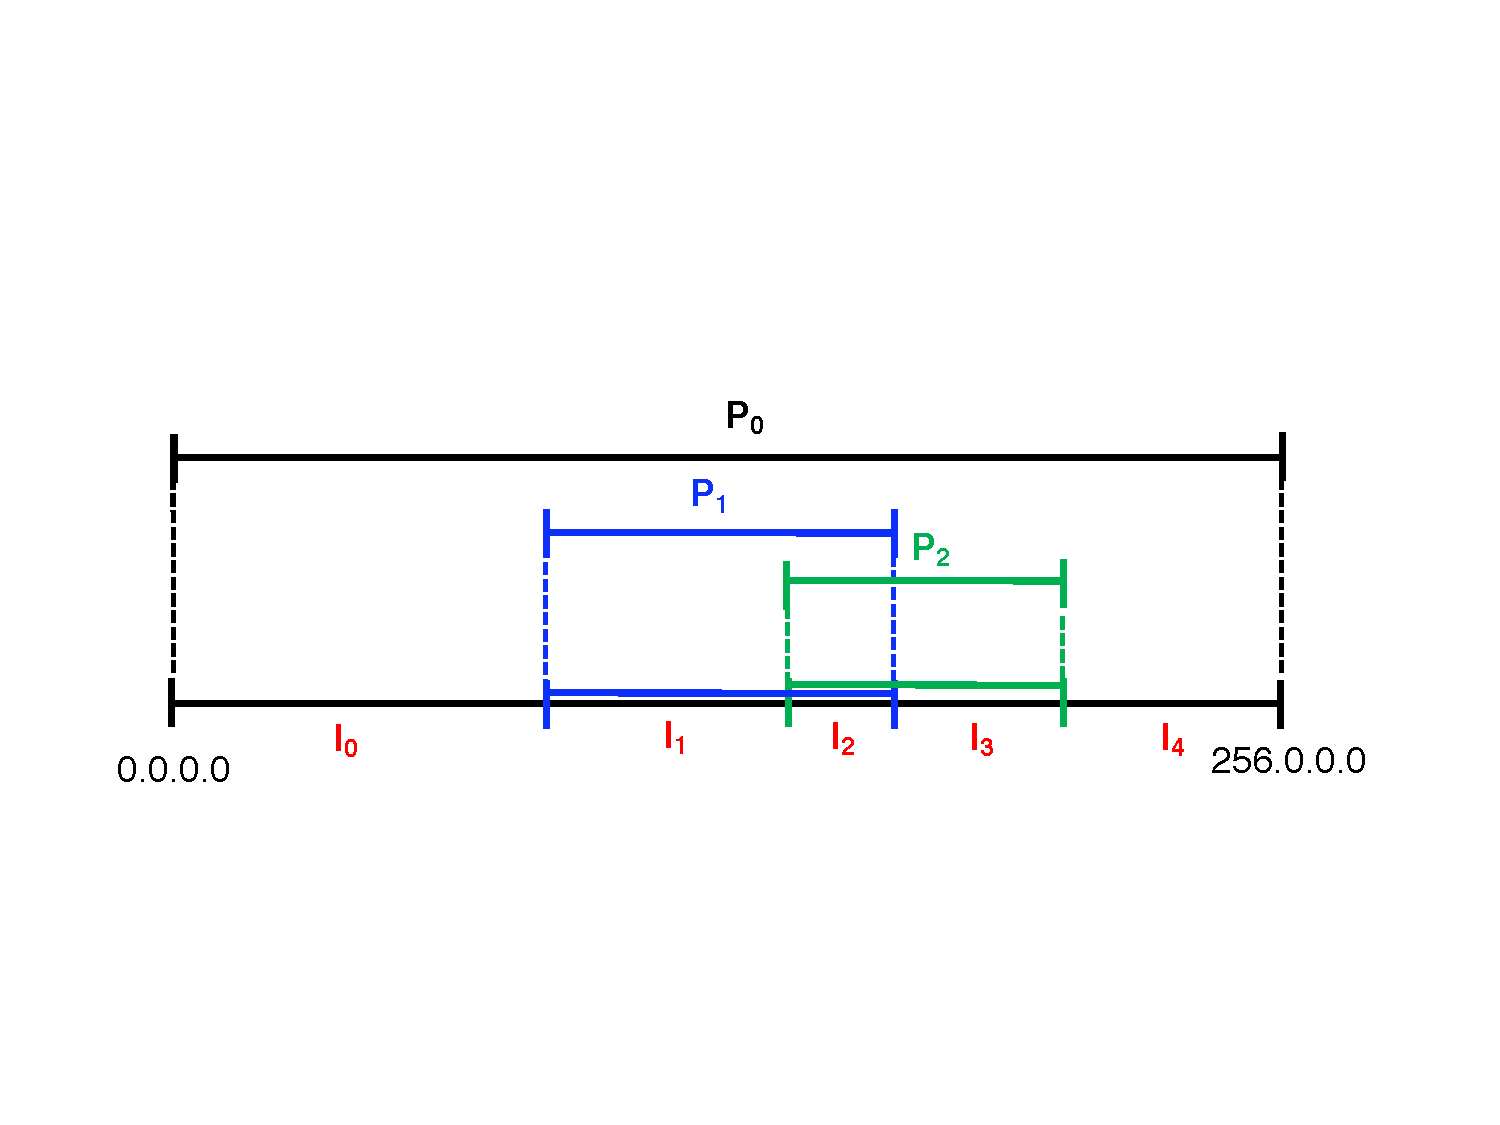
\includegraphics[width=3in]{fig/rangeopts3.pdf}
  \caption[]{Interval map: R2 has higher priority than R1, and the prefixes for intervals are randomly assigned.\label{fig:rangeopts3}}
\end{figure}

To encrypt the ranges $[s_1, e_1)$, $\dots$, $[s_n, e_n)$ with different priorities, what we want to do is equivalent to solving the following problem: given a set of overlapping 1-D line segments of different colors situated at different heights, draw the lines as seen from the top. Hence, PrefixMatch solves this problem by the Bentley-Ottmann algorithm~\cite{bentley}. First, it maps ranges to a random permutation of prefixes. Then, it sorts the endpoints (including 0.0.0.0 and hypothetical 256.0.0.0) into $\mu_1, \mu_2, \dots, \mu_{2n}$ and 
sweeps from left to right. As it sweeps, it maintain a list of ranges that intersect the current position as well as the range with the highest priority. For example, in Fig.~\ref{fig:rangeopts3}, we obtain 4 intervals from 2 ranges R1 and R2. The interval marked with blue refers to R1, while the one marked with yellow refers to R2. Therefore, we have the mapping from intervals to original ranges. Given the mapping from ranges to the random permutation of prefixes that we obtained at the beginning, we then map the intervals to prefixes.

For now, consider that the gateway maintains a mapping of each interval to its assigned prefix, called the {\em interval map}. When the gateway needs to encrypt an IP address $v$, the gateway first determines what is the interval $v$ falls in. It uses the interval map to determine the prefix of the encryption. Then, to obtain the remaining part of the encryption, it uses a pseudorandom function $\prf^n(v)$, mapping $v$ to a random value in the interval 0..n-1. We seed $\prf$ in $q$, a function of both the key and hash of the 5-tuple connection header ($q = \prf_k(\text{conn})$). Note that, in the system setup with two gateways, the gateways generate the same encryption because they share $k$. Let $N$ be $2^{w-m}$, where the value is $w$-bit and the prefix is $m$-bit. The encryption of $v$ is

\begin{equation}
\Enc(v) = \prefix \Vert \prf_q^N(v)
\end{equation}

For example, if $v$ is 127.0.0.1, a possible encryption given the ranges encrypted above is 78.124.24.85. The encryption does not retain any information about $v$ other than the range it is in. In particular, for two values $v_1$ and $v_2$ that match the same interval, their order can be arbitrary. Thus, this satisfies the security requirement above.

The scheme supports NATs -- which require that every time a value for the same connection is encrypted, it returns the same value. It generates a random encryption using a deterministic function. 

When encrypting IP addresses, we do not want two different IP addresses to map to the same encryption (which would break the NAT). Fortunately, the probability that two IP addresses get assigned to the same encryption is negligibly low for IPv6.  The reason is that each interval of prefixes is large because we distributed the endpoints evenly and because there is a small number of such endpoints in a realistic setting (e.g., a firewall has less than 100,000 rules). Suppose we have $n$ distinct rules, $m$ flows and a $w$-bit space, with the assumption of uniformly distributed flows, the probability of getting collision is approximately 

\begin{equation}
1 - e^\frac{-m^2 (2n+1)}{2^{w+1}}
\end{equation}

Therefore, if $w=128$ (which is the case when we use IPv6), the probability is negligible in a normal setting. 

%\begin{figure}
%  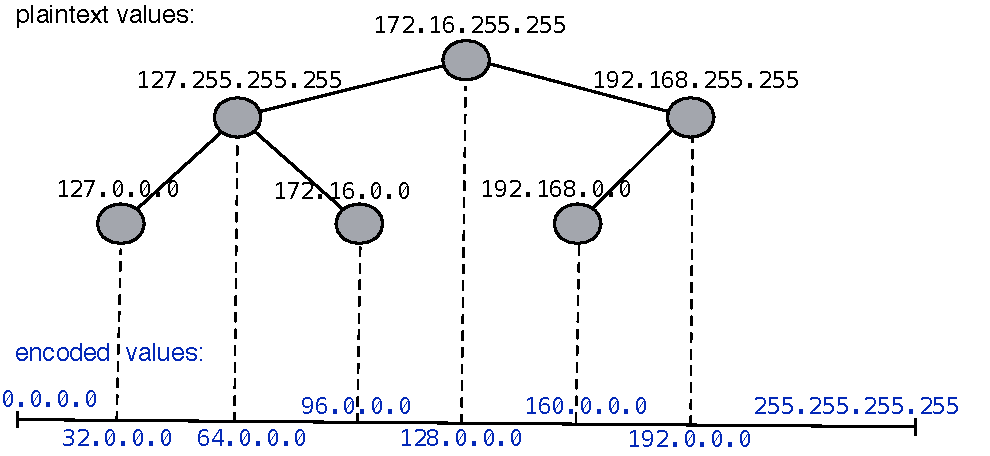
\includegraphics[width=3.25in]{fig/tree}
%  \caption{\label{fig:tree} PrefixMatch tree. The values of nodes in the tree are the %unencrypted IP addresses, and the blue values on the horizontal axis are their encryptions. }
%\end{figure}

\noindent \textbf{Comparing encrypted values against rules.}
The prefixes from the interval map are deployed as new rules on the firewall. It can run prefix matching between any encrypted value $\enc(v)$ and a prefix, and will obtain a correct answer. Comparing $\enc(v_1)$ and $\enc(v_2)$ that match the same prefix is meaningless, and returns a random value.

\noindent \textbf{Handling overlapping ranges.} 
Overlapping ranges share some intervals. Since ranges must have different priorities (e.g. longest prefix matching prefers rules with longer prefixes), we can always break the tie. If a value $\enc(v)$ matches a prefix of one of those intervals, it matches the range with the highest priority.

\noindent \textbf{Updating ranges.}
Adding a new range or removing an existing range with a high priority would affect the intervals it covers. Therefore, in the worst case $O(N)$ rules needs to be updated. 

\subsubsection{Implementing PrefixMatch in the Gateway}
\label{sec:tree}

The gateway stores the interval map for encryption, and it maintains no state per IP address encrypted or per connection.

The gateway can use the following functions. EncryptRanges encrypts the initial ranges. Note that some ranges could consist of
one point only, namely $s + 1 = e$. 


\begin{framed}
\begin{algorithmic}[1]

\Procedure{EncryptRanges}{$R_1$, $\dots$, $R_n$}
  \State Let $R_{\infty}$ = ($-\infty$, $\infty$).
  \State Map $R_1$, $\dots$, $R_n$, $R_{\infty}$ to a random permutation of prefixes $P_i$, $\dots$, $P_n$, $P_{\infty}$
  
  \State Let $R_i$ = [$s_i$, $e_i$), sort the values 
              $V = \{s_1, \dots, s_n\}$ 
              $\cup$ $\{e_1, \dots, e_n\}$.
  \State Ranges := \{\}
  \State TopRange := Null, 
  \State Intervals := \{\}
  \State LastEndpoint := $-\infty$
    
  \ForAll{$v_i \in V$}
    \If{$v_i$ is $s_j$ for some $j$}
      \State $R_{top}$ := TopPriority(Ranges)
      \If{$R_j$.priority > $R_{top}$.priority}
        \State $I$ := ((LastEndpoint, $v_i$), $R_{top}$, $P_{top}$)
        \State Intervals.Add($I$)
        \State LastEndpoint := $v_i$
      \EndIf
      \State Ranges.Add($R_j$) 
    \Else
      \State $R_{top}$ := TopPriority(Ranges)
      \If{$R_{top}$ is $R_j$}
        \State $I$ := ((LastEndpoint, $v_i$), $R_{top}$, $P_{top}$)
        \State Intervals.Add($I$)
        \State LastEndpoint := $v_i$
      \EndIf
      \State Ranges.Remove($R_j$)
    \EndIf
  \EndFor
  \State $I$ := ((LastEndpoint, $\infty$), $R_{\infty}$, $P_{\infty}$)
  \State Intervals.Add($I$)
  \State \Return{Intervals}
\EndProcedure

\end{algorithmic}
\end{framed}

We described how to encrypt values matched against ranges in \S\ref{sec:rmscheme}; it requires identifying the interval $I$ for each value. We can compute $I$ efficiently in logarithmic time by doing a binary search. 

% We now describe the procedure for AddRange which adds an interval (deleting an interval is similar). These procedures modify the state at the gateway. To add a range [$s$, $e$], the gateway inserts these values in the tree. If the tree needs to be rebalanced, for each endpoint that changed location in the tree, the gateway records the old and new encrypted value based on the tree in a list $L$. Note that  the number of endpoints that change encryption is $O(\log n)$ amortized worst-case. The gateway then computes the encryption of $s$ and $e$ based on their location in the tree. It sends to SP $\enc(s)$ and $\enc(e)$ along with $L$. 

%Besides the interval added or deleted, a small number
%of other intervals may be moved -- at worst, $O(\log n)$. 
%For these, the algorithm returns the old and new encryption of the interval. 

%
%\begin{framed}
%\begin{algorithmic}[1]
%
%\Procedure{AddRange}{$[s, e]$}
%  \State Insert $s$ and $e$ into the scapegoat tree. If $s=e$, insert the value only once.
%  %	
%  \State Initialize $L$ to be the empty list.
%  \If{tree needs to be rebalanced}
%  	\State Record which nodes change position in the tree during rebalancing, together with 
%	their old and new encryptions. Namely, record	\[L = \{ \en_1 \leftarrow \en^*_1, \dots, \en_m \rightarrow \en^*_m\},\] where $m$ is the number of nodes who changed position in the tree, and $\en_i$ and $\en^*_i$ are the old and new encryption of the $i$-th node that changed position. 
%  \EndIf
%  \State Compute  $\enc(s)$ and $\enc(e)$, the encryptions of $s$ and $e$, as in EncryptRanges.
%   \State \Return{$[\enc(s), \enc(e)], L$}
%\EndProcedure
%
%\end{algorithmic}
%\end{framed}

%  \State Determing the smallest and the largest encryption in the values $[\enc(s), \enc(e)]$ and $L$, and call this $\dirtyrange$.



\subsubsection{Rule Updates at the Cloud}
\label{sec:updates}
At the cloud, PrefixMatch poses two additional challenges to updating rules, both stemming from the fact that a rule update can also change encrypted values within packets.
The first challenge is middlebox state. Consider a NAT with a translation table containing ports and IP addresses for active connections
Adding or removing a rule will modify these values in the PrefixMatch tree, and thus to continue correct processing the NAT state must be updated.
The second challenge is a race condition: when the middlebox adopts a new ruleset while packets encrypted under the old tree are still flowing, these packets will be misclassified as their encryption values are inconsistent with the ruleset being applied. 
The same problem occurs if packets encrypted under the new tree arrive before the new ruleset.

To avoid these problems the gateway and cloud provider do the following. 
When the gateway updates the PrefixMatch tree, it announces to the cloud provider of the pending update, and the middleboxes ship their current state to the gateway to receive the new encryption values.
The gateway then sends a signal to the cloud provider that it is about to `swap in' the new map. 
The cloud provider buffers traffic for a few hundred milliseconds after this signal to allow all old traffic to complete processing at the cloud; it signals to all middleboxes to `swap in' the new rules and state; and finally it releases the new traffic.
Note that all changes to middleboxes are in the {\it control plane} of the middlebox, and require no modifications to the algorithms and operations performed in per-packet processing. 

\subsubsection{Security Guarantees}
The scheme achieves our desired security goal: the only information leaked about a value $v$ encrypted is which ranges it matches. 
In particular, the scheme is not order preserving because it does not leak the order of two encrypted values that match the same range. It is easy to check that the scheme is secure: since the encryption of $v$ is random in the interval $I$, the scheme only leaks the fact that $v$ is in $I$. $I$ is chosen in such a way that the only information about $v$ it encodes is which intervals $v$ matches and which it does not match. 
%
Since the encryption is seeded in a per-connection identifier, correlation attacks between different flows are not possible. 

